

%\documentclass[12pt,a4paper]{article}
\documentclass[tikz]{standalone}

\usepackage[english]{babel}
\usepackage[utf8]{inputenc}
\usepackage{amsfonts,amssymb,amsbsy}
\usepackage{xcolor}

\usepackage{tikz}
\usetikzlibrary{arrows.meta, positioning, quotes, calc, intersections, decorations.pathreplacing}

\begin{document}

	\begin{tikzpicture}
		\tikzset{
			cuboid/.pic={
				\tikzset{%
					every edge quotes/.append style={midway, auto},
					/cuboid/.cd,
					#1
				}
				\draw [every edge/.append style={pic actions, densely dashed, opacity=.5}, pic actions]
				(0,0,0) coordinate (sl) ++(0,\cubescale*\cubey,\cubescale*\cubez/2) coordinate (o)
					-- ++(-\cubescale*\cubex,0,0) coordinate (a) -- ++(0,-\cubescale*\cubey,0) coordinate (b) -- ++(\cubescale*\cubex,0,0) coordinate (c) -- node[midway] (fm) {} cycle
				(o) -- node[midway] (su1) {} ++(0,0,-\cubescale*\cubez) coordinate (d) -- ++(0,-\cubescale*\cubey,0) coordinate (e) -- (c) -- cycle
				(o) -- (a) -- node[midway] (su2) {} ++(0,0,-\cubescale*\cubez) coordinate (f) -- (d) -- cycle
				($(su1)!0.5!(sl)$) node (sc) {}
				($(su1)!0.5!(su2)$) node (uc) {};
				\draw [opacity=0.3] (f) -- ++(0,-\cubescale*\cubey,0) coordinate(g) (g) -- (e) (g) -- (b);
			},
			conv3d/.pic={\pic [fill=green!50!white, opacity=0.8] {cuboid={#1}};},
			conv2d/.pic={\pic [fill=magenta!60!white, opacity=0.8] {cuboid={#1}};},
			conv2dlr/.pic={\pic [fill=cyan!60!white, opacity=0.8] {cuboid={#1}};},
			conv2dr/.pic={\pic [fill=blue!50!white, opacity=0.8] {cuboid={#1}};},
			upsample/.pic={\pic [fill=yellow!80!white, opacity=0.8] {cuboid={#1}};},
			maxpool/.pic={\pic [fill=blue!80!white, opacity=0.8] {cuboid={#1}};},
			dropout/.pic={\pic [fill=pink, opacity=0.8] {cuboid={#1}};},
			myline/.style={draw=black!50!white, line width=0.4mm, rounded corners},
			myarrow/.style={myline, -{Latex[width=0.2cm, length=0.3cm]}},
			imagestyle/.style={transform shape, anchor=south, inner sep=0, outer sep=0},
			fontstyle/.style={font=\Large},
			/cuboid/.search also={/tikz},
			/cuboid/.cd,
			width/.store in=\cubex,
			height/.store in=\cubey,
			depth/.store in=\cubez,
			units/.store in=\cubeunits,
			scale/.store in=\cubescale,
			width=1,
			height=1,
			depth=1,
			units=cm,
			scale=1
		}
	
		% Input images
		\def\yoffset{-3.6}
		\def\xstep{0.7}
		\def\xskip{2}
		\def\imagewidth{2.5cm}
		\begin{scope}[cm={0.5, 0.5, 0.0, 1.0, (0,0)}]
		
			% Tip 1
			\path (0,0,0) coordinate (origin) node[imagestyle] {
\includegraphics[width=\imagewidth]{images/afm_0_0}}
			++(\xstep,-0.5*\xstep,0) coordinate (im2) node[imagestyle] {
\includegraphics[width=\imagewidth]{images/afm_0_1}}
			++(\xskip,-0.5*\xskip,0) coordinate (im3) node[imagestyle] {
\includegraphics[width=\imagewidth]{images/afm_0_8}}
			++(\xstep,-0.5*\xstep,0) node[imagestyle] {
\includegraphics[width=\imagewidth]{images/afm_0_9}};
			\path ($(im2)+(0,2.2,0)$) -- node[auto=false, fontstyle]{\ldots} ($(im3)+(0,2.3,0)$);
			
			% Tip 2
			\path (origin) ++(0,\yoffset) coordinate (tip2) node[imagestyle] {
\includegraphics[width=\imagewidth]{images/afm_1_0}}
			++(\xstep,-0.5*\xstep,0) coordinate (im2) node[imagestyle] {
\includegraphics[width=\imagewidth]{images/afm_1_1}}
			++(\xskip,-0.5*\xskip,0) coordinate (im3) node[imagestyle] {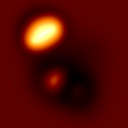
\includegraphics[width=\imagewidth]{images/afm_1_8}}
			++(\xstep,-0.5*\xstep,0) node[imagestyle] {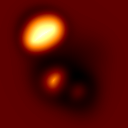
\includegraphics[width=\imagewidth]{images/afm_1_9}};
			\path ($(im2)+(0,2.2,0)$) -- node[auto=false, fontstyle]{\ldots} ($(im3)+(0,2.3,0)$);
			
		\end{scope}
		
		\path (origin) ++(0.8,3.6,0) node[fontstyle] {CO-AFM};
		\path (tip2) ++(0.8,-1.2,0) node[fontstyle] {Xe-AFM};
	
		% Input branches
		\path (origin) ++(3.6,0,0) coordinate (model) pic {conv3d={width=0.4, height=2.5, depth=2.5}}
		++(0.5,0,0) pic {conv3d={width=0.4, height=2.5, depth=2.5}}
		++(0.5,0,0) pic {conv3d={width=0.4, height=2.5, depth=2.5}} (sc) node (c1) {} (sl)
		%
		++(-1.0,\yoffset,0) pic {conv3d={width=0.4, height=2.5, depth=2.5}} (b) node (unet1) {} (sl)
		++(0.5,0,0) pic {conv3d={width=0.4, height=2.5, depth=2.5}}
		++(0.5,0,0) pic {conv3d={width=0.4, height=2.5, depth=2.5}} (sc) node (c2) {};
		
		% Input branch arrows
		\draw[myarrow] (c2) -- ++(1.0, 0);
		\draw[myline] (c1) -- ++(0.55,0) -- ++($(c2)-(c1)$);
	
		% Encoder
		\path ($(sl)+(1.7,0,0)$) pic {conv3d={width=0.4, height=2.5, depth=2.5}}
		++(0.5,0,0) pic {conv3d={width=0.4, height=2.5, depth=2.5}} (uc) node (c3) {} (sl)
		++(0.4,0,0) pic {maxpool={width=0.3, height=2.0, depth=2.0}}
		%
		++(1.2,0,0) pic {conv3d={width=0.3, height=2.0, depth=2.0}}
		++(0.38,0,0) pic {conv3d={width=0.3, height=2.0, depth=2.0}} (uc) node (c4) {} (sl)
		++(0.3,0,0) pic {maxpool={width=0.2, height=1.5, depth=1.5}}
		%
		++(0.9,0,0) pic {conv3d={width=0.2, height=1.5, depth=1.5}}
		++(0.28,0,0) pic {conv3d={width=0.2, height=1.5, depth=1.5}} (uc) node (c5) {} (sl)
		++(0.2,0,0) pic {maxpool={width=0.1, height=1.0, depth=1.0}}
		
		% Middle
		++(0.5,0,0) pic {conv2dlr={width=0, height=1.0, depth=1.0}}
		++(0.15,0,0) pic {conv2dlr={width=0, height=1.0, depth=1.0}}
		++(0.15,0,0) pic {dropout={width=0, height=1.0, depth=1.0}}
		
		% Decoder
		++(0.65,0,0) pic {upsample={width=0, height=1.5, depth=1.5}}
		++(0.15,0,0) pic {conv2dlr={width=0, height=1.5, depth=1.5}}
		++(0.15,0,0) pic {conv2dlr={width=0, height=1.5, depth=1.5}} (uc) node (c6) {} (sl)
		++(0.15,0,0) pic {conv2dlr={width=0, height=1.5, depth=1.5}}
		%
		++(0.8,0,0) pic {upsample={width=0, height=2.0, depth=2.0}}
		++(0.15,0,0) pic {conv2dlr={width=0, height=2.0, depth=2.0}} 
		++(0.15,0,0) pic {conv2dlr={width=0, height=2.0, depth=2.0}} (uc) node (c7) {} (sl)
		++(0.15,0,0) pic {conv2dlr={width=0, height=2.0, depth=2.0}} 
		%
		++(1.1,0,0) pic {upsample={width=0, height=2.5, depth=2.5}}
		++(0.15,0,0) pic {conv2dlr={width=0, height=2.5, depth=2.5}} 
		++(0.15,0,0) pic {conv2dlr={width=0, height=2.5, depth=2.5}} (uc) node (c8) {} (sl)
		++(0.15,0,0) pic {conv2dlr={width=0, height=2.5, depth=2.5}} (sc) node (c9) {};
		
		% Output branch arrows
		\path[myarrow] (c9) -- ++(1.0, 0) coordinate (a);
		\path[myarrow] ($(c9)+(0.55,0,0)$) coordinate (b) -- ++(0,3.6,0) coordinate -- ++($(a)-(b)$);
		
		% Output branches
		\path ($(sl)+(1.3,0,0)$) pic {conv2dlr={width=0, height=2.5, depth=2.5}}
		++(0.15,0,0) pic {conv2dlr={width=0, height=2.5, depth=2.5}} 
		++(0.15,0,0) pic {conv2dr={width=0, height=2.5, depth=2.5}} (c) node (unet2) {} (sl)
		%
		++(-0.3,-\yoffset,0) pic {conv2dlr={width=0, height=2.5, depth=2.5}} 
		++(0.15,0,0) pic {conv2dlr={width=0, height=2.5, depth=2.5}}
		++(0.15,0,0) coordinate (end) pic {conv2d={width=0, height=2.5, depth=2.5}};
		
		% Draw arrow under model
		\path[myarrow] ($(unet1)+(0,0,1)$) -- ++($(unet2)-(unet1)$);
		
		% Output images
		\path (end) ++(2.3,0,0) coordinate (es) node[imagestyle] {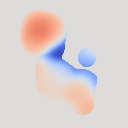
\includegraphics[width=2.8cm]{images/es_map}}
		++(0,\yoffset,0) coordinate (hm) node[imagestyle] {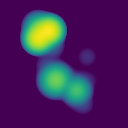
\includegraphics[width=2.8cm]{images/height_map}}
		++(3.6,-\yoffset/2-0.5,0) coordinate (3d) node[imagestyle] {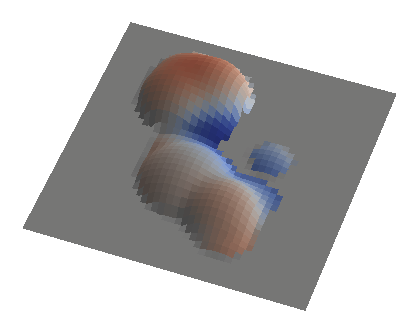
\includegraphics[width=4.0cm]{images/3d}};
		\path (es) ++(0,3.3,0) node[fontstyle] {ES Map};
		\path (hm) ++(0,-0.5,0) node[fontstyle] {Height Map};
		\path (3d) ++(0.2,4.3,0) node[fontstyle, text width=4cm, align=center] {ES Map + Height Map\\3D representation};
		
		% Skip-connection arrows
		\path[myarrow] (c5) -- ++(0.0,0.6,0) -- ++($(c6)-(c5)$) coordinate -- (c6);
		\draw[myarrow] (c4) -- ++(0.0,0.6,0) -- ++($(c7)-(c4)$) coordinate -- (c7);
		\draw[myarrow] (c3) -- ++(0.0,0.6,0) -- ++($(c8)-(c3)$) coordinate -- (c8);
		
		% Legend
		\def\xstep{6.2}
		\def\ystep{-0.7}
		\path (model) ++(2.6,2.7,0) coordinate (start)
		pic {conv3d={width=0.4, height=0.4, depth=0}} ($(fm)+(0.1,-0.03)$) node [fontstyle, right] {3D Conv + LeakyReLU} (sl)
		++(0,\ystep,0) pic {conv2d={width=0.4, height=0.4, depth=0}} ($(fm)+(0.1,0)$) node [fontstyle, right] {2D Conv} (sl)
		++(0,\ystep,0) pic {conv2dlr={width=0.4, height=0.4, depth=0}} ($(fm)+(0.1,-0.05)$) node [fontstyle, right] {2D Conv + LeakyReLU} (sl)
		++(0,\ystep,0) pic {conv2dr={width=0.4, height=0.4, depth=0}} ($(fm)+(0.1,-0.03)$) node [fontstyle, right] {2D Conv + ReLU}
		(start) ++(\xstep,0,0) pic {maxpool={width=0.4, height=0.4, depth=0}} ($(fm)+(0.1,0)$) node [fontstyle, right] {MaxPool} (sl)
		++(0,\ystep,0) pic {upsample={width=0.4, height=0.4, depth=0}} ($(fm)+(0.1,-0.05)$) node [fontstyle, right] {NN upsample} (sl)
		++(0,\ystep,0) pic {dropout={width=0.4, height=0.4, depth=0}} ($(fm)+(0.1,-0.05)$) node [fontstyle, right] {Dropout} (sl);
	
	\end{tikzpicture}
	
	
\end{document}